\begin{surferPage}[Cuintic\u{a} (15 cusp)]{O cuintic\u{a} cu 15 puncte cuspidale}
      Aceast\u{a} suprafa\c{t}\u{a} de grad $5$ (cuintic\u{a}) are $15$ singularit\u{a}\c{t}i de tip $A_2$
    (numite puncte cuspidale). Aceast\u{a} cuintic\u{a}, \^{i}mpreun\u{a} cu o serie de suprafe\c{t}e asem\u{a}n\u{a}toare, 
    au ap\u{a}rut \^{i}ntr-un articol din 2005 al lui Oliver Labs.
    Cinci dintre punctele cuspidale arat\u{a} altfel dec\^{a}t celelalte zece.
    \^{I}ntr-adev\u{a}r, cele cinci sunt de tip $A_2^{++} $, iar restul de tip $A_2^{+ -}$ (vezi
    galeria cu singularit\u{a}\c{t}i simple pentru mai multe informa\c{t}ii):

     \vspace*{-0.3em}
    \begin{center}
      \begin{tabular}{c@{\qquad}c}
        \includegraphics[height=1.2cm]{dessins_quint_15a2}
        &
        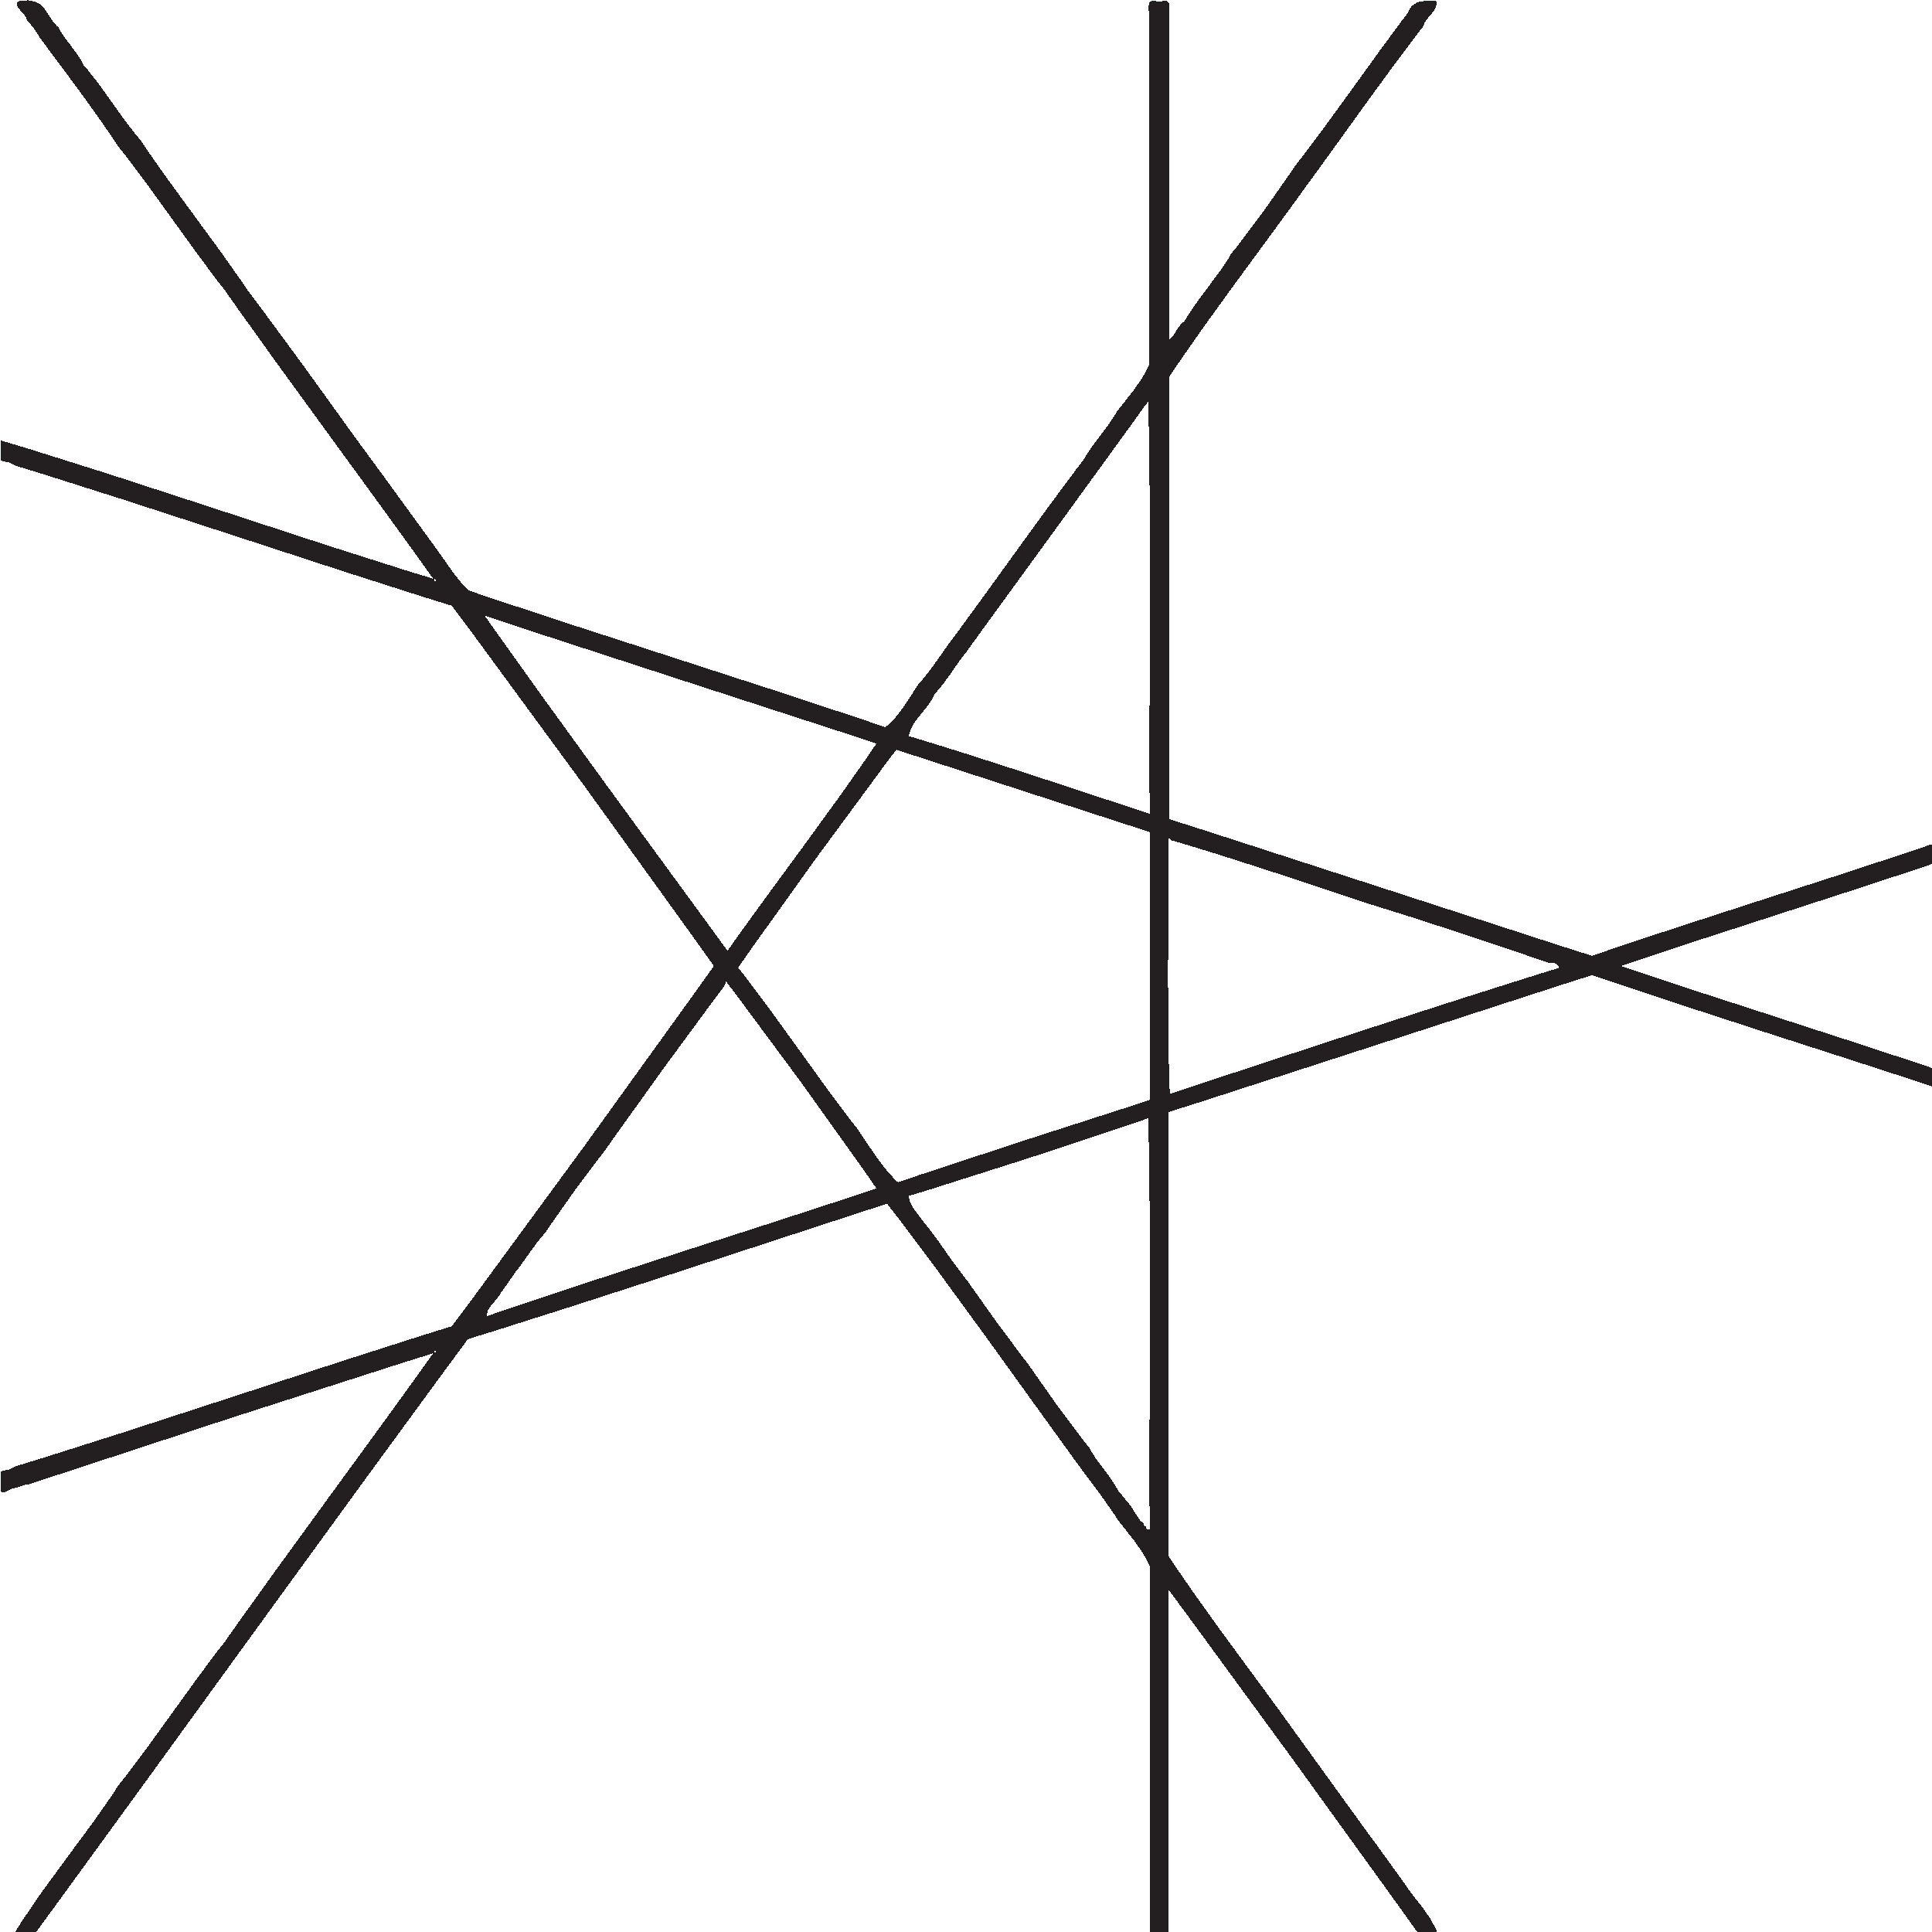
\includegraphics[height=1.2cm]{rp5.pdf}
      \end{tabular}
    \end{center}
    \vspace*{-0.3em}    
    
        Aceast\u{a} suprafa\c{t}\u{a} are o ecua\c{t}ie de forma $S_5(x,y) + t(z)=0,$
    unde $S_5(x,y)$ este un pentagon regulat (imaginea din dreapta), \c{s}i $t(z)$ este
    o variant\u{a} a polinoamelor Chebyshev, pe care le-am mentionat de mai multe ori p\^{a}n\u{a} acum.
    
    O alt\u{a} cuintic\u{a} (st\^{a}nga) cu $15$ puncte cuspidale a fost construit\u{a} de Wolf Barth.
    Este legat\u{a} de cubica lui Clebsch (dreapta), dup\u{a} cum se poate observa din imaginea din mijloc:

    \vspace*{-0.3em}
    \begin{center}
      \begin{tabular}{c@{\quad}c@{\quad}c}
        \includegraphics[height=1.2cm]{barthquintic_green}
        &
        \includegraphics[height=1.2cm]{barthquintic_clebschcubic}
        &
        \includegraphics[height=1.2cm]{clebschcubic_pink}
      \end{tabular}
    \end{center}
    \vspace*{-0.3em}
\end{surferPage}
